\chapter{Evaluation}
\section{Experiments and Measurements}
\subsection{Experiment A: Orchestral Concert to Analyze Musical Absorption using Nidra to Collect Breathing Data}
The experiment was conducted in collaboration with master student Joachim Dalgard at the University of Oslo at the faculty of \textit{RITMO: Centre for Interdisciplinary Studies in Rhythm, Time and Motion}. 

The goal of the experiment was to analyze musical absorption, which is a state an individuals ability and willingness allows music to draw them into an emotional experience and becomes unaware of time and space. In order to analyze the effect of musical absorption on individuals, we gathered 20 participants who were experienced listeners with musical education. The participants attended an orchestral concert by Richard Strauss' Alpine Symphony---a symphonic poem that portrays the experience of eleven hours spent climbing an Alpine mountain---that lasted around 50 minutes at Oslo Concert Hall on third of April and fourth of April 2019.  

However, the motivation for this experiment for our application can be summarized into: (1) to test the application in a real-life and crowded environment, in order to analyze whether other mobile devices interfere or obstruct with the signals between the collecting sensor and the device; (2) to test whether the samples gathered are meaningfull, in the sense that the application is collecting the samples from the sensors correctly, and handling unexpected disconnections; and (3) to test the application on different Android OS versions, and to put the application in the hands of participants. 

The participants were divided into two groups to attend the concert on the two dates. Each participant was equipped with a wireless electromyographic sensor from DELSYS in order to measure heart rate, and a Flow sensor kit to measure respiration during the concert. RITMO had multiple Flow sensors for disposal; however, they had no suitable mobile application that could record with these sensors. Also, with their equipment they experienced that Flow sensor kits tended to disconnect every 10-15 minutes, resulting in fragmented recordings for a single session. Therefore, they reached out to \textit{Insitute for Informatics} in hopes of a solution. Our application was a suiting match for both parties, hence a collaboration was formed [? do i need this]. We arranged for six Android devices and reached out to the participants to bring their Android devices if they had one. There were ten participants in each group and six assessed devices. As a precaution, we decided to give out the devices to the participants who scored highest on a test performed on beforehand.

During the concert, there were approximately 800 attendees on the first day and approximately 1500 attendees on the second day. We assume that most of the attendees had a mobile device, and a few shares of them had BlueTooth activated on the device. Based on these estimates, we were able to replicate an environment (on a larger scale) where other devices might interfere with the signals between the collecting sensor and the application. Also, we were able to install the application on multiple mobile devices with different Android OS versions and put the application in the hands of the participants. 




\subsubsection{Preperations}

\begin{table}
\begin{center}
\scalebox{0.59}{
\begin{tabular}{ |c|c|c|c| } 
\hline
\textbf{Model} & \textbf{Samsung Galaxy S9} & \textbf{OnePlus 3T} & \textbf{Google Pixel XL} \\
\hline
Operating System & Android 8.0 & - & Android 9.0 \& Android 7.1.2  \\
Chipset & Exynos 9810  & Qualcomm MSM8996 Snapdragon 821 & Qualcomm MSM8996 Snapdragon 821  \\
CPU & Octa-core & Quad-core & Quad-core \\
GPU & Mali-G72 MP18 & Adreno 530 & Adreno 530  \\
RAM & 4 GB & 6 GB & 4 GB \\
Battery & Li-Ion 3000 mAh & Li-Ion 3400 mAh & Li-Ion 3450 mAh  \\
Bluetooth & 5.0, A2DP, LE, aptX & 4.2, A2DP, aptX HD, LE & 4.2, A2DP, LE, aptX \\

\hline
\end{tabular}}
\caption{Device models used during the concert}
\end{center}
\end{table}

In order to partake in the experiments, we had to ensure that the participant had the sensor placed accurately on their body and the mobile devices were configured correctly. Additional tests were also performed in order to ensure the application worked as intended, and also to prevent any unforeseen events or bugs that could have occurred during the recording. 

\begin{description}
    \item[Device Configuration] The device models in our disposal had to be configured with the applications to enable recording on Nidra. First, the data stream dispatching module was installed on the devices. Second, the sensor wrapper for the Flow sensor kit was configured with one Flow sensor on beforehand---in order to reduce the time to set up the mobile device and the sensor on the participant before the concert. Lastly, the Nidra application was initiated with a unique name (A-F), as such to distinguish each participant with the sensor and device model. In Figure 6.1, the device models are listed with their specifications and the OS ... [Skriv mer]
    \item[Body Placement] The respiration value is based on the participant body circumference, and changes are associated with breathing. The participant was instructed to place the sensor around their thorax (just below the armpits), in order to measure the expansion and contraction of the rib cage.

\end{description}

\subsubsection{Results}

We gathered all of the recordings from the various devices by using the sharing functionality in the application and sent it to our application. There were thirteen mobile devices combined for both dates---one of the participants had an Android device---however, the application crashed on one of the mobile devices during the recording. Therefore, we have access to twelve recordings from the concerts. 

\begin{figure}
\parbox{7cm}{
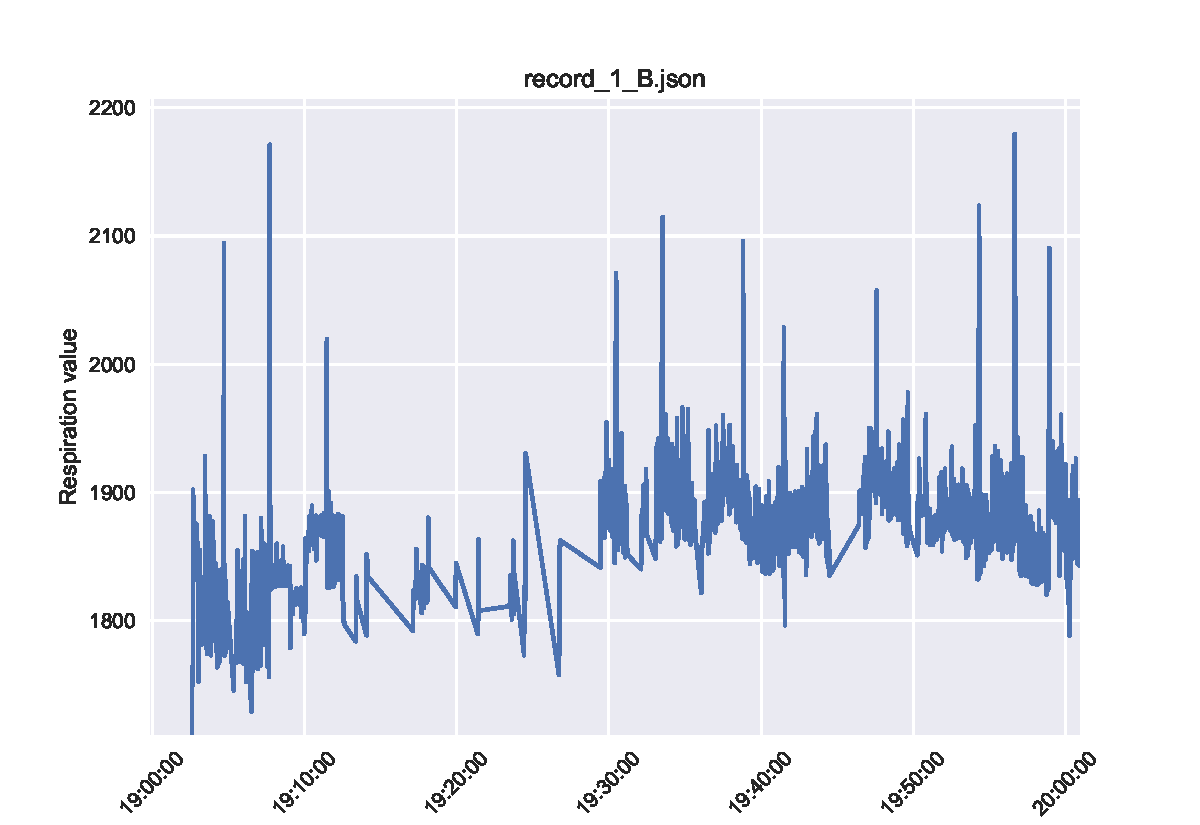
\includegraphics[width=8cm]{images/Record_1_B.pdf}
\caption{Concert Day 1---Mobile Device B}
\label{fig:day_1}}
\qquad
\begin{minipage}{6cm}
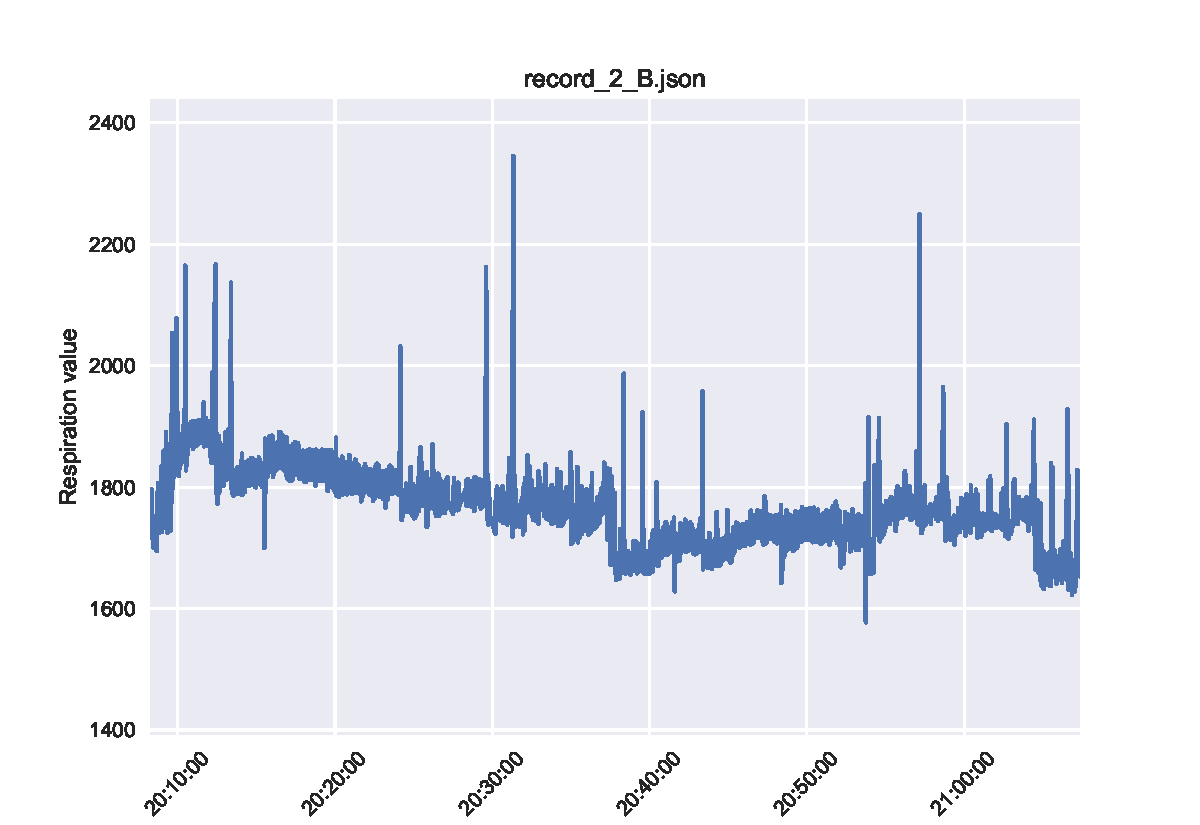
\includegraphics[width=7cm]{images/Record_2_B.pdf}
\caption{Concert Day 2---Mobile Device B}
\label{fig:day_2}
\end{minipage}
\end{figure}

Figure \ref{fig:day_1} and Figure \ref{fig:day_2} present two of these twelve recordings (rest can is found in Appendix B) that are of most interest to us in a time-series graph. The Y-axis represents the respiration (breathing) value, and the X-axis the time of respiration value acquisition---\textit{day one} of the concert started at the time of 19:00 and ended at 20:00, while \textit{day two} started at the time of 20:10 and ended 21:00. The graphs are plotted with Python and the library MatPlotLib in order to analyze and evaluate the sample values; however, an identical graph is also presented in the application.

From the thesis "..." by Løberg, we can group the signals strengths based on four types of breathing patterns: (1) normal breathing---normal exhaling and inhaling (12-18 breaths per minute); (2) no breathing---close to flat rates over a long period; (3) shallow breathing---rapid inhaling and exhaling; and (4) deep breathing---prolonged inhaling or exhaling (also denoted as fluctuations). From the Figures, we can see that the respiration value is stable with some fluctuations and disconnections. Disconnections are defined as when the line is sloping or benching in an extended period (e.g., 20 seconds or more), while fluctuations are samples that spikes (deep breathing) in the graph. We should keep in mind that the margin for the normal breathing respiration value can vary throughout the recording based on body or sensor position and movements (e.g., sitting relax or tense in a chair). 

Figure 6.1 has many disconnections (further analyzed later) with unstable breathing. There are multiple occurrences of deep breathing throughout the recording, with some shallow breathing at the start and the end of the recording. Hypothetically, deep breathing might be a sign of musical absorption; however, we have no concrete analysis of this matter, and it is out of the scope for this experiment motivation. Moving on, Figure 6.2 shows fewer disconnects compared to Figure 6.1, and with much more concise breathing patterns and resemblance to normal breathing. Although, there are noticably deep breathing throughout the recording, with a few shallow breathings at the beginning. Conclusively, both Figures shows no nuances for no breathing during the recording. However, there are signs of normal breathing, with few instances of shallow and deep breathing. 

\subsubsection{Analysis \& Discussion}
We will discuss all twelve records by analyzing the respiration values. It is of special interest to find occurrences of disconnections---when the samples are stagnant in more extended period---and the time the sensor is disconnected during the recording.

\begin{table}[!h]
\begin{center}
\scalebox{0.7}{
\begin{tabular}{ |c|c|c|c||c|c| } 
\hline
\textbf{Model} & \textbf{Samples Count} & \textbf{Loss Count} & \textbf{Loss Percentage} & \textbf{Disconnection Count} & \textbf{Disconnection Time} \\
\hline
A & 5145 & 0 & 0 \% & 0  & 00:00  \\
\hline
B & 3363 & 1782 & 34 \% & 13 & 19m:14s  \\
\hline
C & 4189 & 956 & 19 \% & 7 & 8m:20s  \\
\hline
D & 3501 & 1644 & 32 \% & 5 & 18m:30s  \\
\hline
E & 5144 & 1 & 0.02 \% & 0 & 00:00  \\
\hline
F & 5145 & 0  & 0 \% & 0 & 00:00  \\
\hline
\end{tabular}}
\caption{Day 1---Duration: 1 hour \& Roof Samples: 5145}
\end{center}
\end{table}


\begin{table}[!h]
\begin{center}
\scalebox{0.7}{
\begin{tabular}{ |c|c|c|c||c|c| } 
\hline
\textbf{Model} & \textbf{Samples Count} & \textbf{Loss Count} & \textbf{Loss Percentage} & \textbf{Disconnection Count} & \textbf{Disconnection Time} \\
\hline
A & 4286 & 2 & 0.05 \% & 0  & 00:00  \\
\hline
B & 4161 & 127 & 3 \% & 4 & 1m:25s  \\
\hline
C & 4286 & 2 & 0.05 \% & 0 & 00:00  \\
\hline
D & 2576 & 1712 & 40 \% & 7 & 24m:35s  \\
\hline
E & 4285 & 3 & 0.06 \% & 0 & 00:00  \\
\hline
F & 4288 & 0  & 0 \% & 0 & 00:00  \\
\hline
\end{tabular}}
\caption{Day 2---Duration: 50 mins. \& Roof Samples: 4288}
\end{center}
\end{table}

The recordings for the six devices for the two dates are represented in Table 6.2 and Table 6.3. Each table exhibits data that is extracted from each recording from the mobile device and can be characterized as: 

\begin{description}
    \item[Roof Sample] The expected number of samples that can be acquired in the period of the recording (based on the frequency of sample output by Flow Sensor).
    \item[Sample Count] The number of samples that were gathered in the duration of the recording. 
    \item[Loss Count] The number of missing samples based on \verb|Roof Samples|. This can be calculated as: 
\begin{equation} \label{losscount}
Loss\ Count = Roof\ Samples - Samples\ Count
\end{equation}
    \item[Loss Percentage] The percentage of missing samples based on the expected samples. This can be calculated as:
\begin{equation} \label{losscount}
Loss\ Percentage = (1 - \frac{Samples\ Count}{Roof\ Samples}) * 100
\end{equation}
    \item[Disconnection Count] Is the number of disconnections that occurred within the duration of the recording.
    \item[Disconnection Time] Is the accumulated time of disconnection. 
\end{description}

The device models A, E, and F are noticeably accurate (with some noises which presumably occurred during parsing), there are no apparent disconnects occurred during the recording for these models both of the days. In contrast, device model B, C, D shows an outburst of disconnections during recording. Especially, model D has high loss percentage both of the days, which is reflected in the disconnection time. Also, model B had a high loss percentage on the first day; however, significantly less loss percentage the second day. Similar resemblance can also be seen in model C.

We could conclude on the fact that some mobile device models or some sensors is malfunctioned, and for this reason we see higher loss rate. Unfortunately, with insufficent data to point out whether that is correct, is is something we cannot conclude on. Moreover, [Skriv mer om Android OS version].

\subsubsection{Conclusion}
To summarize the experiment, we were able to test the application in a real-life and crowded environment. The application managed to record samples that lasted up to 1 hour with the Flow senor and various device models with different Android OS versions. However, one of the application crashed, and we were unable to find the source of the problem. Based on samples from the recording, it is identified that the Flow sensor has a tendency of disconnecting, but the application managed to provide a continuous data stream by reconnecting with the sensor during recording. In the end, the records were successfully shared across applications, which enabled us to analyze the recordings.  

To conclude, the goal of the experiment was to analyze musical absorption during a concert, but that is not the motivation for our application. However, we provided an application that collected the data during the concert. Thus, the collected data can then be used to conclude a correlation between breathing and musical absorption. Also, inconsistency in the sampling of the recordings makes it difficult to determine the source of the problem. We could argue that the analysis of the aggregated data in the tables might indicate that the sensor or the mobile is a malfunctioned, however, due to insufficient data this conclusion cannot be drawn. Although, the application managed to collect data with the use of the Flow sensor kit, in an environment filled with other mobile devices that could have interfered with the signals, as well as reconnecting to the sensors during the recording. [Reflect more on the motivation goals].

\subsection{Experiment B: 8-hours recording}

\subsection{Experiment C: Performing User-Tests on Two Participants}
One goal of the application is that it should be user-friendly enough for patients to use and understand how the functionality of our application works. To evaluate whether this goal has been achieved, we found two participants that agreed to partake in the experiment. One of these participants is not proficent in the use of modern technology, while the other participant has a lot of experience. For simplicity, we will refer to the participant as participant \verb|A| and \verb|B|, respectively. 

The testing process consisted of three parts: a presentation of the application, tests to record and share the recording, and an interview. The tests were not performed during the night, due to ... However, this tests focuses on user-friendliness, rather than recording over an extended period. The participant was informed with the scinario the application was designed for. 

\begin{description}
    \item[Presentation] We presented the goal and the functionality of the application to the participants in a simple and intuity way. However, we mainly focused on explaining the recording functionality and the methods of sharing the recording across applications. The presentation was took around 10 minutes, including questions and clarifications.  
    \item[Tests] The tests were mainly desgined to evaluate comprehensibility and usability in the application. Comprehensibility is to evalute the participants ability to understand the functionality of the application, while usability to measure ease of use of the application.
    \item[Interview] The interview was conducted after thes tests were performed, so the participant had their feedback fresh in memory. We structured the questions in the interview accordingly to the PACMAD methodology. 
\end{description}

\subsubsection{Testing}
To evaluate whether the application presents the functionality adequently and suffice the goal of the tests, we tested the participants with certain tasks:
\begin{itemize}
    \item[T1] Proceed to navigate in the application and start a recording.
    \item[T2] Find the interface to check for connected sensor sources, and the graph for the sampling
    \item[T3] Stop the recording, and finialize the recording session by giving it a name, description and rating.
    \item[T4] Find the recording in the feed of recordings. 
    \item[T5] Share the recording over e-email.
    \item[T6] View the analytics for the recording by interacting with it (e.g., zooming and scrolling). 
\end{itemize}

For this test to be successful, the participants must for all of the tasks be able to correctly identify the actions. There were no interference or guidance on how to perform the tests, besides guiding the participants into performing each task. These tests were designed to observe and simulate the primary actions the user mainly focuses on in the application. Thus, the functionality of modules and importing recordings were left behind. 


\subsubsection{Observations}
Participants \verb|A|---less technical---had to familiarize with the setting of the application, thus had a hard start to begin with. It took the participant longer than exepected to perform T1, however, managed to proceed on recording and was bit uncertain whether the recording had started or not. Also, the participant was flabbergasted by the rippling effect the recording screen presented. The T2 was somewhat tedious to perform, because the participant tried to click on the interface where it says it should be expanded (by swiping). Also, the graph was bit hard to interact with because the interface above the graph kept moving while performing interactions with the graph. T3 and T4 went fine, the participant filled out the title, description and a rating and saved the recording, and find the recording on the feed screen. However, the T5 and T6 was bit unclear to the participant, because the functionality is hidden, and in order to find the actions you have to press the record to expand the information. However, after that was clear, the participant managed to perform both task sufficently. 

Participants \verb|B| outperformed participant \verb|A|, due to the participent were more fimilar with technical systems. The participant managed to start the recording quickly, however, were unsure whether the recording had starting (clicking around on the interface for feedback), untill the ripple effects appeared on the screen. Similar to participant A, participant B clicked on the interface for statistics, rather than swiping. Also, had a hard time to interact with the graph due to the interface moving. The particpent B managed to perform T3-T6 with ease and without any interupts or objections. 


\subsubsection{Discussion}

Conclusively, the tests were not performed to its desired intent, due to the fiddeling in on the recording screen. However, the participant managed to perform most of the tasks regardless, albeit the task T1 and T2 were hard to comprehend. 

Both of the participants had a hard time to understand whether the sensor was collecting data, despite the ripple effects on the screen. Argueably, the user can familiaries with the state of the recording and the ripple effects which indicates sample acquestion, however, to a new user that is bit hard to time understand this. The source of this problem is that the sensor takes some time (i.e., 30-60 seconds) to output the samples, however, the sensor establishment between Nidra and the sensor wrapper occurres imediately. 

Also, the interface to view for expanding the statistics was bit tedeous to understand. 

Besides this, there we no noticably complains by the participant. They found the color scheme of the application to be smooth and fitting, and the application to be moderen. Also, they find stuff to be well organized and were not drowned in selections and actions to perform. All of the functionality is restricted to few and simple actions per screen. 

\subsubsection{Survey}
The interview questions were performed after the tasks. The questions followed a PACMAD survey structure, which is a model to identify the usability attributes and are structed into: effectiveness, efficency, statisfaction, learnability, memorability, errors, and cogitive load. We created a survey based on some of the structure, however, we were unable to perform any cogitive load or memoriability tasks during the testing. Hence, the participant filled out the questions regarding: 

\noindent \textbf{Effectiveness \& Efficency}
\begin{itemize}
    \item What were your inital thoughts on the application
    
    \begin{description}[font=\normalfont\itshape]
        \item[Participent A:] The application looked nice and simple-
        \item[Participent B:] 
    \end{description}
    

    \item How difficult was it to start a recording (very hard (1)--very easy (5))
    
    \begin{description}[font=\normalfont\itshape]
        \item[Participent A:] 1
        \item[Participent B:] 3
    \end{description}

    \item How would you rate the feedback you got during a recording (very bad (1)--very good (5))
    \begin{description}[font=\normalfont\itshape]
        \item[Participent A:] 2
        \item[Participent B:] 3
    \end{description}

    \item How difficult was it to stop a recording? (very hard (1)--very easy (5))
    \begin{description}[font=\normalfont\itshape] 
        \item[Participent A:] 5
        \item[Participent B:] 5
    \end{description}
    \item How difficult was to browse/find previous recordings? (very hard (1)--very easy (5))
    \begin{description}[font=\normalfont\itshape]
        \item[Participent A:] 3
        \item[Participent B:] 5
    \end{description}
    \item Did you have any encounters were the application did not supply you with enough information?
    \begin{description}[font=\normalfont\itshape]
        \item[Participent A:]
        \item[Participent B:] 
    \end{description}
\end{itemize}

\noindent \textbf{Satisfaction}

\begin{itemize}
    \item How satisfied were you with the "journey"? (not satisfied (1)--very satistifed (5))
    \begin{description}[font=\normalfont\itshape]
        \item[Participent A:] 3
        \item[Participent B:] 3
    \end{description}
    \item How satisfied were you with this application overall? (Not satisifed (1)--very satisfied (5))
    \begin{description}[font=\normalfont\itshape]
        \item[Participent A:] 4
        \item[Participent B:] 4 
    \end{description}
\end{itemize}

\noindent \textbf{Errors}

\begin{itemize}
    \item If you encountered any crashes or errors during the time you used the application, please answer the question below.
    \begin{description}[font=\normalfont\itshape]
        \item[Participent A:] None.
        \item[Participent B:] None.
    \end{description}

\end{itemize}

\noindent \textbf{Feedback and Improvements}

\begin{itemize}
    \item How user friendly did you find the application to be? (Not so friendly (1)--Very friendly (5))
    \begin{description}[font=\normalfont\itshape]
        \item[Participent A:] 4
        \item[Participent B:] 4
    \end{description}
    \item How would you rate the color palette of the application? (Not so pleasing colors (1)--Very pelasing colors (5))
    \begin{description}[font=\normalfont\itshape]
        \item[Participent A:] 5
        \item[Participent B:] 5
    \end{description}
    \item How would you rate the general layout of the application (buttons, text, navigation, etc...)? (Very bad (1)--Very good (5))
    \begin{description}[font=\normalfont\itshape]
        \item[Participent A:] 4
        \item[Participent B:] 5
    \end{description}
    \item Do you have any feedback/improvements to the application itself?
    \begin{description}[font=\normalfont\itshape]
        \item[Participent A:]
        \item[Participent B:] 
    \end{description}
\end{itemize}


\subsubsection{Conlusions}

\subsection{Experiment D: Creating a Simple Module}
One of the goals of the application is to provide an interface for the developers to create modules, which allows for data enrichment and extended functionality. In order to test for this, we found one participant that had experience in software development, and with some experience in Android development. The tests was for the participant to create a new module in our application, which utilized the records in order to find the record that has the highest number of samples. The development of a user-interface was not evaluted, thus displaying the correct answer on the screen was sufficent. 

Before the the participant started on creating a new module, an simple introduction on the concepts and data was performed. Mainly, the fact that Nidra formats the all of the data (e.g., records and corresponding samples) into a JSON string, and the JSON string is put into a bundle with the key \textit{data}, and sent up on launching the module-application (with Intent). The data structure were also introduced, i.e., an array of records with meta-data and correlated samples.

\subsubsection{Process}

The participent created a new Android project named \textit{TestModule}. For the simplicity, all of the development occurred in one activity. The first task was to get the JSON string that was bundled on launch in an Intent with the key of \textit{data}. The second task was to decode the data, the participant used  \verb|Gson| library in order to parse the data accordingly to the struture. And the final task was to display the results, which the participant did by iterating through the records and finding the one with the highest sample count.

\subsubsection{Observations}
Despite the tasks seemlingly looks easy of making a simple module, the participant had a rough start. The participant was aware that module-application received data in a bundle, and the extraction could . However, for each time the participant compiled, the module-application crashed. That is because the bundle is empty if the module-application is launched directly, and not through the Nidra application (while supplies the module with the data). Albeit, the participant managed to handle this error early. 

The next challenge for the participant was to understand how to transform the JSON string into valid objects in Java. First, the participant had to create an object which encapsulates the record and and a list of samples (\verb|ExportObject|). Then, three seperate objects (i.e., record, sample, and user) had to be created, that were identical to the payload. As such, the participant could decode the JSON string into an list of the \verb|ExportObject|, and retrieve the necessary data.

Once the participant had all of the data, the rest of the tasks was simily accomplished. THe participant iterated through the list of records, and found the one with the highest sample count, and displayed it on the screen. 

\subsubsection{Results}

In Figure X, the module-application is illustrated. As of the experiement, there were five records on the mobile device---and the highest was the record named \verb|Record 17| with \verb|163| samples---thus, the experiement was successful conducted. It took the participant approximately 30 minutes to develop this module-application, where most of the time went to parse the data.

\subsubsection{Discussion \& Conlusion}

Conclusively, the participant managed to create a module, with some hurdles in the way. Noticably, while compling the project the participant had to open its module through the Nidra application in order to get the data. There are two ways to prevent this from happening, one way is to establish an IPC (discueed in the design chapther) with the use of an AIDL file and output the data from Nidra to the application through the IPC connection. The second way is to cache the data in the module-application, for temporary storage of the data. However, both methods increases the complexity of the module-application. Nonetheless, the former improvement can be made in Nidra.

The second noticable occurances, was the the parsing of the JSON data. JSON is a bit tedeous to work with in Java. As of now, there is no direct support for parsing JSON in Java, hence third-party libraries has to be used in order to do so. To combat the start-up face of a new module-application, we will include boilplate code (found in Appendix C), to make module implementation easily comprehenceable for future developers.


%Any changes commited in the module or Nidra, is not reflected with each other. When changing the code in the module application, 

\section{Main Findings}
